\begin{frame}
	\frametitle{Length of Exploration Phase}
	
	\begin{columns}[c]
		
		\column{.45\textwidth}

		\begin{itemize}
			\item compare landscape features ever 10\%
			\item using Euclidean distance
			\item trade-off between
				\begin{itemize}
					\item time for exploration
					\item time for adjusted configuration
				\end{itemize}
			\item between 20 and 40\% from search (percentage of classification)
		\end{itemize}
		
		\column{.45\textwidth}
		\begin{figure}
			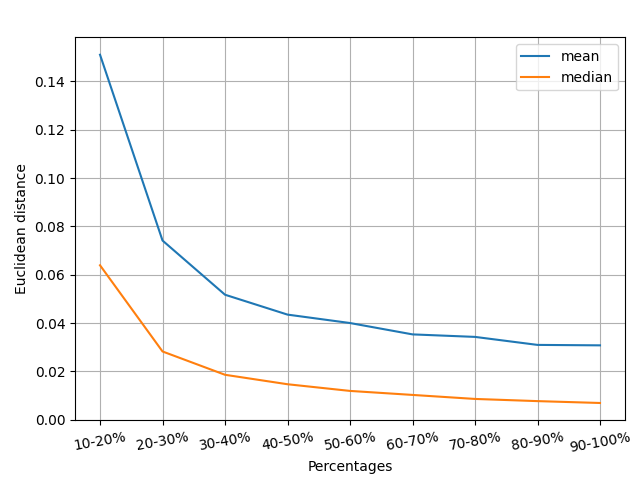
\includegraphics[width=1\textwidth]{figures/euclidean_distances}
		\end{figure}
		
		
	\end{columns}
	
\end{frame}

\begin{frame}
	\frametitle{Machine learning algorithm}
	
	\begin{itemize}
		\item binary classification
		\item supervised learning
		\item fast classification
		\item few features
		\item decision tree
	\end{itemize}
	
\end{frame}

\begin{frame}
	\frametitle{Hyper-parameter search}
	
	\begin{itemize}
		\item only apply on as many as possible
			\begin{itemize}
				\item TPR > 80\%
			\end{itemize}
		\item only apply if positive effect
			\begin{itemize}
				\item FPR < 5\%
			\end{itemize}
		\item percentage of classification (POC)
		\item construction criteria (Gini Impurity, Entropy or Log-Loss)
		\item depth of decision tree
	\end{itemize}
	
\end{frame}

\begin{frame}
	\frametitle{Component selection}
	
	\begin{columns}[c]
		
		\column{.45\textwidth}
		\blockheading{Decision tree}
		
		\begin{itemize}
			\item $stdev > 0.1 \& cov. max(cov.) * 0.8$
			\item depth of decision tree: 2
			\item Gini Impurity
			\item POC: 30\%
		\end{itemize}
		
		\column{.45\textwidth}		
		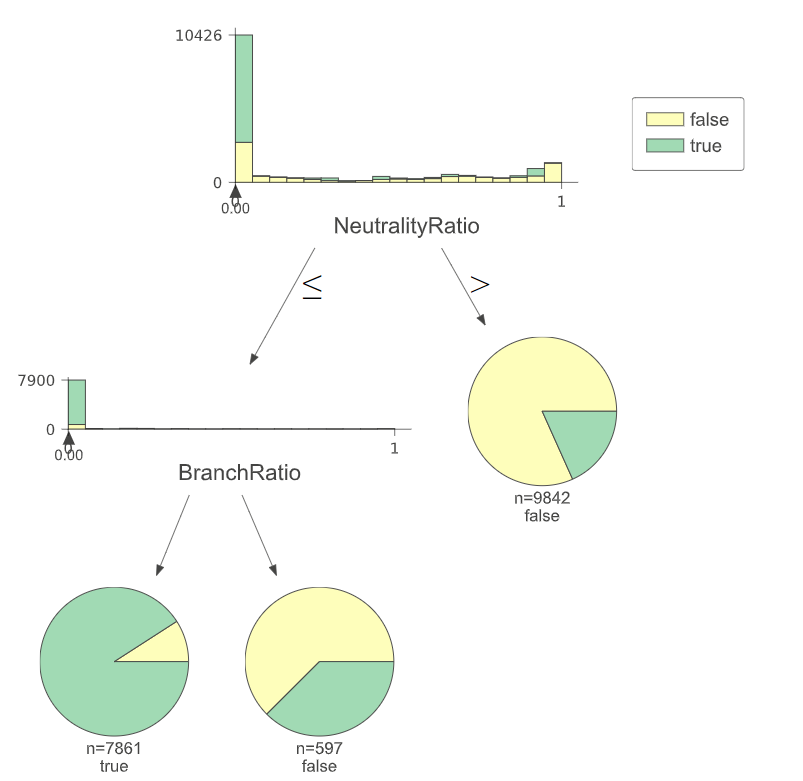
\includegraphics[height=0.8\textheight]{figures/decision_tree}
		
	\end{columns}
	
	
\end{frame}